% Venue-neutral IEEE-style draft (IEEEtran). Retarget by swapping the document class and the abstract/introduction/conclusion files.
% TITLE IS A DRAFT: the evaluation-protocol framing follows the post-hoc sensitivity result; confirm before submission.
% All numbers come from generated/numbers.tex (paper/make_numbers.py) so the text cannot drift from results/.
% DRAFT: simulation only, pre-validation. No hardware results exist; hardware appears only as a replication plan (Appendix A).
\documentclass[conference]{IEEEtran}
\usepackage{amsmath,amssymb,booktabs,graphicx,siunitx,hyperref,cite,multirow}
\graphicspath{{../generated/}}
% generated by paper/make_numbers.py - do not edit
\newcommand{\ConfThreeChangesBanditMean}{+1.19}
\newcommand{\ConfThreeChangesBanditMed}{+0.17}
\newcommand{\ConfThreeChangesCap}{24}
\newcommand{\ConfThreeChangesCapMean}{10}
\newcommand{\ConfThreeChangesGainKdBase}{1.32}
\newcommand{\ConfThreeChangesGainKdMed}{1.78}
\newcommand{\ConfThreeChangesGainKdPhi}{1.87}
\newcommand{\ConfThreeChangesGainKdPlo}{1.48}
\newcommand{\ConfThreeChangesGainKiBase}{0.00}
\newcommand{\ConfThreeChangesGainKiMed}{0.00}
\newcommand{\ConfThreeChangesGainKiPhi}{9.00}
\newcommand{\ConfThreeChangesGainKiPlo}{0.00}
\newcommand{\ConfThreeChangesGainKpBase}{29.59}
\newcommand{\ConfThreeChangesGainKpMed}{27.23}
\newcommand{\ConfThreeChangesGainKpPhi}{35.83}
\newcommand{\ConfThreeChangesGainKpPlo}{23.59}
\newcommand{\ConfThreeChangesHi}{+1.23}
\newcommand{\ConfThreeChangesInfBase}{-85.5}
\newcommand{\ConfThreeChangesInfOrc}{-42.6}
\newcommand{\ConfThreeChangesInfPpo}{-85.2}
\newcommand{\ConfThreeChangesLo}{+0.24}
\newcommand{\ConfThreeChangesMean}{+1.53}
\newcommand{\ConfThreeChangesMed}{+0.58}
\newcommand{\ConfThreeChangesMhi}{+2.15}
\newcommand{\ConfThreeChangesMlo}{+1.04}
\newcommand{\ConfThreeChangesN}{83}
\newcommand{\ConfThreeChangesNInf}{17}
\newcommand{\ConfThreeChangesOrcAbs}{6.48}
\newcommand{\ConfThreeChangesOrcPct}{34}
\newcommand{\ConfThreeChangesQone}{$-$0.15}
\newcommand{\ConfThreeChangesQthree}{+2.69}
\newcommand{\ConfThreeChangesSeedAHolm}{0.0057}
\newcommand{\ConfThreeChangesSeedAMed}{+0.54}
\newcommand{\ConfThreeChangesSeedBHolm}{1.9e-05}
\newcommand{\ConfThreeChangesSeedBMed}{+0.58}
\newcommand{\ConfThreeChangesSeedCHolm}{1}
\newcommand{\ConfThreeChangesSeedCMed}{+0.32}
\newcommand{\ConfThreeChangesSelected}{ppo\_s1}
\newcommand{\ConfThreeChangesSucc}{37}
\newcommand{\ConfThreeChangesSuccBase}{27}
\newcommand{\ConfThreeCommit}{72c1219963}
\newcommand{\ConfThreeOodBanditMean}{+0.45}
\newcommand{\ConfThreeOodBanditMed}{$-$0.05}
\newcommand{\ConfThreeOodCap}{46}
\newcommand{\ConfThreeOodCapMean}{31}
\newcommand{\ConfThreeOodGainKdBase}{1.32}
\newcommand{\ConfThreeOodGainKdMed}{1.78}
\newcommand{\ConfThreeOodGainKdPhi}{1.87}
\newcommand{\ConfThreeOodGainKdPlo}{1.55}
\newcommand{\ConfThreeOodGainKiBase}{0.00}
\newcommand{\ConfThreeOodGainKiMed}{0.00}
\newcommand{\ConfThreeOodGainKiPhi}{0.00}
\newcommand{\ConfThreeOodGainKiPlo}{0.00}
\newcommand{\ConfThreeOodGainKpBase}{23.67}
\newcommand{\ConfThreeOodGainKpMed}{27.83}
\newcommand{\ConfThreeOodGainKpPhi}{34.88}
\newcommand{\ConfThreeOodGainKpPlo}{23.57}
\newcommand{\ConfThreeOodHi}{+0.74}
\newcommand{\ConfThreeOodInfBase}{-35.5}
\newcommand{\ConfThreeOodInfOrc}{-34.7}
\newcommand{\ConfThreeOodInfPpo}{-35.0}
\newcommand{\ConfThreeOodLo}{+0.24}
\newcommand{\ConfThreeOodMean}{+1.05}
\newcommand{\ConfThreeOodMed}{+0.45}
\newcommand{\ConfThreeOodMhi}{+1.38}
\newcommand{\ConfThreeOodMlo}{+0.74}
\newcommand{\ConfThreeOodN}{91}
\newcommand{\ConfThreeOodNInf}{9}
\newcommand{\ConfThreeOodOrcAbs}{2.27}
\newcommand{\ConfThreeOodOrcPct}{26}
\newcommand{\ConfThreeOodQone}{+0.02}
\newcommand{\ConfThreeOodQthree}{+1.51}
\newcommand{\ConfThreeOodSeedAHolm}{4.6e-09}
\newcommand{\ConfThreeOodSeedAMed}{+0.30}
\newcommand{\ConfThreeOodSeedBHolm}{7.3e-11}
\newcommand{\ConfThreeOodSeedBMed}{+0.45}
\newcommand{\ConfThreeOodSeedCHolm}{3.7e-10}
\newcommand{\ConfThreeOodSeedCMed}{+0.32}
\newcommand{\ConfThreeOodSelected}{ppo\_s1}
\newcommand{\ConfThreeOodSucc}{56}
\newcommand{\ConfThreeOodSuccBase}{47}
\newcommand{\ConfThreeSelStepA}{400}
\newcommand{\ConfThreeSelStepB}{340}
\newcommand{\ConfThreeSelStepC}{30}
\newcommand{\ConfThreeStaticBanditMean}{+0.69}
\newcommand{\ConfThreeStaticBanditMed}{$-$0.09}
\newcommand{\ConfThreeStaticCap}{60}
\newcommand{\ConfThreeStaticCapMean}{43}
\newcommand{\ConfThreeStaticGainKdBase}{1.32}
\newcommand{\ConfThreeStaticGainKdMed}{1.78}
\newcommand{\ConfThreeStaticGainKdPhi}{1.88}
\newcommand{\ConfThreeStaticGainKdPlo}{1.53}
\newcommand{\ConfThreeStaticGainKiBase}{0.00}
\newcommand{\ConfThreeStaticGainKiMed}{0.00}
\newcommand{\ConfThreeStaticGainKiPhi}{0.00}
\newcommand{\ConfThreeStaticGainKiPlo}{0.00}
\newcommand{\ConfThreeStaticGainKpBase}{18.94}
\newcommand{\ConfThreeStaticGainKpMed}{27.82}
\newcommand{\ConfThreeStaticGainKpPhi}{35.37}
\newcommand{\ConfThreeStaticGainKpPlo}{23.51}
\newcommand{\ConfThreeStaticHi}{+0.75}
\newcommand{\ConfThreeStaticInfBase}{-39.5}
\newcommand{\ConfThreeStaticInfOrc}{-37.7}
\newcommand{\ConfThreeStaticInfPpo}{-38.5}
\newcommand{\ConfThreeStaticLo}{+0.29}
\newcommand{\ConfThreeStaticMean}{+1.14}
\newcommand{\ConfThreeStaticMed}{+0.61}
\newcommand{\ConfThreeStaticMhi}{+1.50}
\newcommand{\ConfThreeStaticMlo}{+0.83}
\newcommand{\ConfThreeStaticN}{91}
\newcommand{\ConfThreeStaticNInf}{9}
\newcommand{\ConfThreeStaticOrcAbs}{1.90}
\newcommand{\ConfThreeStaticOrcPct}{26}
\newcommand{\ConfThreeStaticQone}{+0.08}
\newcommand{\ConfThreeStaticQthree}{+1.69}
\newcommand{\ConfThreeStaticSeedAHolm}{1.4e-06}
\newcommand{\ConfThreeStaticSeedAMed}{+0.23}
\newcommand{\ConfThreeStaticSeedBHolm}{1.1e-12}
\newcommand{\ConfThreeStaticSeedBMed}{+0.61}
\newcommand{\ConfThreeStaticSeedCHolm}{3.5e-15}
\newcommand{\ConfThreeStaticSeedCMed}{+0.40}
\newcommand{\ConfThreeStaticSelected}{ppo\_s1}
\newcommand{\ConfThreeStaticSucc}{58}
\newcommand{\ConfThreeStaticSuccBase}{49}
\newcommand{\ConfThreeValDegA}{0.00}
\newcommand{\ConfThreeValDegB}{0.07}
\newcommand{\ConfThreeValDegC}{0.57}
\newcommand{\ExplThreeChangesCap}{20}
\newcommand{\ExplThreeChangesCapMean}{11}
\newcommand{\ExplThreeChangesHi}{+1.49}
\newcommand{\ExplThreeChangesInfBase}{-115.3}
\newcommand{\ExplThreeChangesInfOrc}{-44.0}
\newcommand{\ExplThreeChangesInfPpo}{-123.3}
\newcommand{\ExplThreeChangesLo}{+0.25}
\newcommand{\ExplThreeChangesMean}{+1.47}
\newcommand{\ExplThreeChangesMed}{+0.55}
\newcommand{\ExplThreeChangesMhi}{+2.55}
\newcommand{\ExplThreeChangesMlo}{+0.56}
\newcommand{\ExplThreeChangesN}{89}
\newcommand{\ExplThreeChangesNInf}{11}
\newcommand{\ExplThreeChangesOrcAbs}{7.37}
\newcommand{\ExplThreeChangesOrcPct}{35}
\newcommand{\ExplThreeChangesQone}{$-$0.15}
\newcommand{\ExplThreeChangesQthree}{+2.66}
\newcommand{\ExplThreeChangesSeedAHolm}{2.4e-05}
\newcommand{\ExplThreeChangesSeedAMed}{+0.57}
\newcommand{\ExplThreeChangesSeedBHolm}{9e-05}
\newcommand{\ExplThreeChangesSeedBMed}{+0.55}
\newcommand{\ExplThreeChangesSeedCHolm}{0.54}
\newcommand{\ExplThreeChangesSeedCMed}{+0.35}
\newcommand{\ExplThreeChangesSelected}{ppo\_s1}
\newcommand{\ExplThreeChangesSucc}{44}
\newcommand{\ExplThreeChangesSuccBase}{34}
\newcommand{\ExplThreeCommit}{72c1219963}
\newcommand{\ExplThreeOodCap}{52}
\newcommand{\ExplThreeOodCapMean}{34}
\newcommand{\ExplThreeOodHi}{+0.96}
\newcommand{\ExplThreeOodInfBase}{-57.3}
\newcommand{\ExplThreeOodInfOrc}{-57.0}
\newcommand{\ExplThreeOodInfPpo}{-57.1}
\newcommand{\ExplThreeOodLo}{+0.26}
\newcommand{\ExplThreeOodMean}{+1.06}
\newcommand{\ExplThreeOodMed}{+0.57}
\newcommand{\ExplThreeOodMhi}{+1.34}
\newcommand{\ExplThreeOodMlo}{+0.81}
\newcommand{\ExplThreeOodN}{94}
\newcommand{\ExplThreeOodNInf}{6}
\newcommand{\ExplThreeOodOrcAbs}{2.03}
\newcommand{\ExplThreeOodOrcPct}{19}
\newcommand{\ExplThreeOodQone}{+0.07}
\newcommand{\ExplThreeOodQthree}{+1.84}
\newcommand{\ExplThreeOodSeedAHolm}{1.1e-08}
\newcommand{\ExplThreeOodSeedAMed}{+0.29}
\newcommand{\ExplThreeOodSeedBHolm}{1.2e-11}
\newcommand{\ExplThreeOodSeedBMed}{+0.57}
\newcommand{\ExplThreeOodSeedCHolm}{2.9e-13}
\newcommand{\ExplThreeOodSeedCMed}{+0.42}
\newcommand{\ExplThreeOodSelected}{ppo\_s1}
\newcommand{\ExplThreeOodSucc}{69}
\newcommand{\ExplThreeOodSuccBase}{49}
\newcommand{\ExplThreeStaticCap}{59}
\newcommand{\ExplThreeStaticCapMean}{38}
\newcommand{\ExplThreeStaticHi}{+0.83}
\newcommand{\ExplThreeStaticInfBase}{-57.5}
\newcommand{\ExplThreeStaticInfOrc}{-57.1}
\newcommand{\ExplThreeStaticInfPpo}{-57.2}
\newcommand{\ExplThreeStaticLo}{+0.30}
\newcommand{\ExplThreeStaticMean}{+0.83}
\newcommand{\ExplThreeStaticMed}{+0.50}
\newcommand{\ExplThreeStaticMhi}{+1.02}
\newcommand{\ExplThreeStaticMlo}{+0.66}
\newcommand{\ExplThreeStaticN}{94}
\newcommand{\ExplThreeStaticNInf}{6}
\newcommand{\ExplThreeStaticOrcAbs}{1.40}
\newcommand{\ExplThreeStaticOrcPct}{18}
\newcommand{\ExplThreeStaticQone}{+0.10}
\newcommand{\ExplThreeStaticQthree}{+1.48}
\newcommand{\ExplThreeStaticSeedAHolm}{1.4e-05}
\newcommand{\ExplThreeStaticSeedAMed}{+0.20}
\newcommand{\ExplThreeStaticSeedBHolm}{2.6e-13}
\newcommand{\ExplThreeStaticSeedBMed}{+0.50}
\newcommand{\ExplThreeStaticSeedCHolm}{1.1e-15}
\newcommand{\ExplThreeStaticSeedCMed}{+0.37}
\newcommand{\ExplThreeStaticSelected}{ppo\_s1}
\newcommand{\ExplThreeStaticSucc}{74}
\newcommand{\ExplThreeStaticSuccBase}{54}
\newcommand{\PaperCommit}{dae93216ae}
\newcommand{\VFourPpoChangesCap}{-7}
\newcommand{\VFourPpoChangesCapMean}{-10}
\newcommand{\VFourPpoChangesGainKdBase}{1.32}
\newcommand{\VFourPpoChangesGainKdMed}{1.23}
\newcommand{\VFourPpoChangesGainKdPhi}{1.24}
\newcommand{\VFourPpoChangesGainKdPlo}{1.21}
\newcommand{\VFourPpoChangesGainKiBase}{0.00}
\newcommand{\VFourPpoChangesGainKiMed}{0.00}
\newcommand{\VFourPpoChangesGainKiPhi}{0.00}
\newcommand{\VFourPpoChangesGainKiPlo}{0.00}
\newcommand{\VFourPpoChangesGainKpBase}{29.59}
\newcommand{\VFourPpoChangesGainKpMed}{19.53}
\newcommand{\VFourPpoChangesGainKpPhi}{19.75}
\newcommand{\VFourPpoChangesGainKpPlo}{19.40}
\newcommand{\VFourPpoChangesHi}{+0.43}
\newcommand{\VFourPpoChangesInfBase}{-64.8}
\newcommand{\VFourPpoChangesInfOrc}{-37.7}
\newcommand{\VFourPpoChangesInfPpo}{-72.4}
\newcommand{\VFourPpoChangesLo}{$-$0.08}
\newcommand{\VFourPpoChangesMean}{$-$0.49}
\newcommand{\VFourPpoChangesMed}{+0.18}
\newcommand{\VFourPpoChangesMhi}{+0.18}
\newcommand{\VFourPpoChangesMlo}{$-$1.28}
\newcommand{\VFourPpoChangesN}{86}
\newcommand{\VFourPpoChangesNInf}{14}
\newcommand{\VFourPpoChangesOrcAbs}{6.99}
\newcommand{\VFourPpoChangesOrcPct}{35}
\newcommand{\VFourPpoChangesQone}{$-$0.52}
\newcommand{\VFourPpoChangesQthree}{+0.77}
\newcommand{\VFourPpoChangesSeedAHolm}{1.5e-10}
\newcommand{\VFourPpoChangesSeedAMed}{$-$1.20}
\newcommand{\VFourPpoChangesSeedBHolm}{1}
\newcommand{\VFourPpoChangesSeedBMed}{+0.13}
\newcommand{\VFourPpoChangesSeedCHolm}{1}
\newcommand{\VFourPpoChangesSeedCMed}{+0.18}
\newcommand{\VFourPpoChangesSelected}{ppo\_s2}
\newcommand{\VFourPpoChangesSucc}{40}
\newcommand{\VFourPpoChangesSuccBase}{36}
\newcommand{\VFourPpoCommit}{50313602cf}
\newcommand{\VFourPpoOodCap}{17}
\newcommand{\VFourPpoOodCapMean}{6}
\newcommand{\VFourPpoOodGainKdBase}{1.32}
\newcommand{\VFourPpoOodGainKdMed}{1.23}
\newcommand{\VFourPpoOodGainKdPhi}{1.24}
\newcommand{\VFourPpoOodGainKdPlo}{1.21}
\newcommand{\VFourPpoOodGainKiBase}{0.00}
\newcommand{\VFourPpoOodGainKiMed}{0.00}
\newcommand{\VFourPpoOodGainKiPhi}{0.00}
\newcommand{\VFourPpoOodGainKiPlo}{0.00}
\newcommand{\VFourPpoOodGainKpBase}{23.67}
\newcommand{\VFourPpoOodGainKpMed}{19.58}
\newcommand{\VFourPpoOodGainKpPhi}{19.81}
\newcommand{\VFourPpoOodGainKpPlo}{19.46}
\newcommand{\VFourPpoOodHi}{+0.36}
\newcommand{\VFourPpoOodInfBase}{-38.3}
\newcommand{\VFourPpoOodInfOrc}{-37.4}
\newcommand{\VFourPpoOodInfPpo}{-38.3}
\newcommand{\VFourPpoOodLo}{+0.29}
\newcommand{\VFourPpoOodMean}{+0.31}
\newcommand{\VFourPpoOodMed}{+0.34}
\newcommand{\VFourPpoOodMhi}{+0.47}
\newcommand{\VFourPpoOodMlo}{+0.14}
\newcommand{\VFourPpoOodN}{93}
\newcommand{\VFourPpoOodNInf}{7}
\newcommand{\VFourPpoOodOrcAbs}{1.79}
\newcommand{\VFourPpoOodOrcPct}{20}
\newcommand{\VFourPpoOodQone}{+0.25}
\newcommand{\VFourPpoOodQthree}{+0.57}
\newcommand{\VFourPpoOodSeedAHolm}{5.8e-06}
\newcommand{\VFourPpoOodSeedAMed}{$-$0.56}
\newcommand{\VFourPpoOodSeedBHolm}{2e-08}
\newcommand{\VFourPpoOodSeedBMed}{+0.30}
\newcommand{\VFourPpoOodSeedCHolm}{2.5e-08}
\newcommand{\VFourPpoOodSeedCMed}{+0.34}
\newcommand{\VFourPpoOodSelected}{ppo\_s2}
\newcommand{\VFourPpoOodSucc}{66}
\newcommand{\VFourPpoOodSuccBase}{63}
\newcommand{\VFourPpoSelStepA}{150}
\newcommand{\VFourPpoSelStepB}{20}
\newcommand{\VFourPpoSelStepC}{60}
\newcommand{\VFourPpoStaticCap}{27}
\newcommand{\VFourPpoStaticCapMean}{11}
\newcommand{\VFourPpoStaticGainKdBase}{1.32}
\newcommand{\VFourPpoStaticGainKdMed}{1.23}
\newcommand{\VFourPpoStaticGainKdPhi}{1.24}
\newcommand{\VFourPpoStaticGainKdPlo}{1.21}
\newcommand{\VFourPpoStaticGainKiBase}{0.00}
\newcommand{\VFourPpoStaticGainKiMed}{0.00}
\newcommand{\VFourPpoStaticGainKiPhi}{0.00}
\newcommand{\VFourPpoStaticGainKiPlo}{0.00}
\newcommand{\VFourPpoStaticGainKpBase}{18.94}
\newcommand{\VFourPpoStaticGainKpMed}{19.58}
\newcommand{\VFourPpoStaticGainKpPhi}{19.81}
\newcommand{\VFourPpoStaticGainKpPlo}{19.47}
\newcommand{\VFourPpoStaticHi}{+0.36}
\newcommand{\VFourPpoStaticInfBase}{-42.3}
\newcommand{\VFourPpoStaticInfOrc}{-40.4}
\newcommand{\VFourPpoStaticInfPpo}{-42.0}
\newcommand{\VFourPpoStaticLo}{+0.34}
\newcommand{\VFourPpoStaticMean}{+0.38}
\newcommand{\VFourPpoStaticMed}{+0.35}
\newcommand{\VFourPpoStaticMhi}{+0.40}
\newcommand{\VFourPpoStaticMlo}{+0.36}
\newcommand{\VFourPpoStaticN}{93}
\newcommand{\VFourPpoStaticNInf}{7}
\newcommand{\VFourPpoStaticOrcAbs}{1.40}
\newcommand{\VFourPpoStaticOrcPct}{19}
\newcommand{\VFourPpoStaticQone}{+0.33}
\newcommand{\VFourPpoStaticQthree}{+0.39}
\newcommand{\VFourPpoStaticSeedAHolm}{1.9e-06}
\newcommand{\VFourPpoStaticSeedAMed}{$-$0.62}
\newcommand{\VFourPpoStaticSeedBHolm}{1.6e-15}
\newcommand{\VFourPpoStaticSeedBMed}{+0.33}
\newcommand{\VFourPpoStaticSeedCHolm}{1.6e-15}
\newcommand{\VFourPpoStaticSeedCMed}{+0.35}
\newcommand{\VFourPpoStaticSelected}{ppo\_s2}
\newcommand{\VFourPpoStaticSucc}{67}
\newcommand{\VFourPpoStaticSuccBase}{66}
\newcommand{\VFourPpoValDegA}{0.13}
\newcommand{\VFourPpoValDegB}{0.18}
\newcommand{\VFourPpoValDegC}{0.69}
\newcommand{\VFourSacChangesCap}{-23}
\newcommand{\VFourSacChangesCapMean}{-26}
\newcommand{\VFourSacChangesHi}{$-$0.06}
\newcommand{\VFourSacChangesInfBase}{-64.8}
\newcommand{\VFourSacChangesInfOrc}{-37.7}
\newcommand{\VFourSacChangesInfPpo}{-58.7}
\newcommand{\VFourSacChangesLo}{$-$1.14}
\newcommand{\VFourSacChangesMean}{$-$1.57}
\newcommand{\VFourSacChangesMed}{$-$0.26}
\newcommand{\VFourSacChangesMhi}{$-$0.86}
\newcommand{\VFourSacChangesMlo}{$-$2.39}
\newcommand{\VFourSacChangesN}{86}
\newcommand{\VFourSacChangesNInf}{14}
\newcommand{\VFourSacChangesOrcAbs}{6.99}
\newcommand{\VFourSacChangesOrcPct}{35}
\newcommand{\VFourSacChangesQone}{$-$2.37}
\newcommand{\VFourSacChangesQthree}{+0.12}
\newcommand{\VFourSacChangesSeedAHolm}{0.00041}
\newcommand{\VFourSacChangesSeedAMed}{$-$0.26}
\newcommand{\VFourSacChangesSeedBHolm}{5.2e-07}
\newcommand{\VFourSacChangesSeedBMed}{$-$0.97}
\newcommand{\VFourSacChangesSeedCHolm}{4.2e-08}
\newcommand{\VFourSacChangesSeedCMed}{$-$1.40}
\newcommand{\VFourSacChangesSelected}{sac\_s0}
\newcommand{\VFourSacChangesSucc}{37}
\newcommand{\VFourSacChangesSuccBase}{36}
\newcommand{\VFourSacCommit}{50313602cf}
\newcommand{\VFourSacOodCap}{-2}
\newcommand{\VFourSacOodCapMean}{-12}
\newcommand{\VFourSacOodHi}{+0.29}
\newcommand{\VFourSacOodInfBase}{-38.3}
\newcommand{\VFourSacOodInfOrc}{-37.4}
\newcommand{\VFourSacOodInfPpo}{-38.1}
\newcommand{\VFourSacOodLo}{+0.19}
\newcommand{\VFourSacOodMean}{$-$0.03}
\newcommand{\VFourSacOodMed}{+0.24}
\newcommand{\VFourSacOodMhi}{+0.18}
\newcommand{\VFourSacOodMlo}{$-$0.28}
\newcommand{\VFourSacOodN}{93}
\newcommand{\VFourSacOodNInf}{7}
\newcommand{\VFourSacOodOrcAbs}{1.79}
\newcommand{\VFourSacOodOrcPct}{20}
\newcommand{\VFourSacOodQone}{$-$0.02}
\newcommand{\VFourSacOodQthree}{+0.37}
\newcommand{\VFourSacOodSeedAHolm}{0.029}
\newcommand{\VFourSacOodSeedAMed}{+0.24}
\newcommand{\VFourSacOodSeedBHolm}{1}
\newcommand{\VFourSacOodSeedBMed}{+0.07}
\newcommand{\VFourSacOodSeedCHolm}{0.0081}
\newcommand{\VFourSacOodSeedCMed}{$-$0.21}
\newcommand{\VFourSacOodSelected}{sac\_s0}
\newcommand{\VFourSacOodSucc}{60}
\newcommand{\VFourSacOodSuccBase}{63}
\newcommand{\VFourSacSelStepA}{20}
\newcommand{\VFourSacSelStepB}{10}
\newcommand{\VFourSacSelStepC}{10}
\newcommand{\VFourSacStaticCap}{4}
\newcommand{\VFourSacStaticCapMean}{-10}
\newcommand{\VFourSacStaticHi}{+0.32}
\newcommand{\VFourSacStaticInfBase}{-42.3}
\newcommand{\VFourSacStaticInfOrc}{-40.4}
\newcommand{\VFourSacStaticInfPpo}{-41.4}
\newcommand{\VFourSacStaticLo}{+0.12}
\newcommand{\VFourSacStaticMean}{+0.05}
\newcommand{\VFourSacStaticMed}{+0.25}
\newcommand{\VFourSacStaticMhi}{+0.28}
\newcommand{\VFourSacStaticMlo}{$-$0.18}
\newcommand{\VFourSacStaticN}{93}
\newcommand{\VFourSacStaticNInf}{7}
\newcommand{\VFourSacStaticOrcAbs}{1.40}
\newcommand{\VFourSacStaticOrcPct}{19}
\newcommand{\VFourSacStaticQone}{$-$0.29}
\newcommand{\VFourSacStaticQthree}{+0.41}
\newcommand{\VFourSacStaticSeedAHolm}{0.47}
\newcommand{\VFourSacStaticSeedAMed}{+0.25}
\newcommand{\VFourSacStaticSeedBHolm}{1}
\newcommand{\VFourSacStaticSeedBMed}{+0.08}
\newcommand{\VFourSacStaticSeedCHolm}{0.0011}
\newcommand{\VFourSacStaticSeedCMed}{$-$0.24}
\newcommand{\VFourSacStaticSelected}{sac\_s0}
\newcommand{\VFourSacStaticSucc}{56}
\newcommand{\VFourSacStaticSuccBase}{66}
\newcommand{\VFourSacValDegA}{2.49}
\newcommand{\VFourSacValDegB}{0.28}
\newcommand{\VFourSacValDegC}{2.22}
\newcommand{\VFourTdChangesCap}{-29}
\newcommand{\VFourTdChangesCapMean}{-44}
\newcommand{\VFourTdChangesHi}{$-$1.82}
\newcommand{\VFourTdChangesInfBase}{-64.8}
\newcommand{\VFourTdChangesInfOrc}{-37.7}
\newcommand{\VFourTdChangesInfPpo}{-54.7}
\newcommand{\VFourTdChangesLo}{$-$2.50}
\newcommand{\VFourTdChangesMean}{$-$2.06}
\newcommand{\VFourTdChangesMed}{$-$2.13}
\newcommand{\VFourTdChangesMhi}{$-$0.72}
\newcommand{\VFourTdChangesMlo}{$-$2.91}
\newcommand{\VFourTdChangesN}{86}
\newcommand{\VFourTdChangesNInf}{14}
\newcommand{\VFourTdChangesOrcAbs}{6.99}
\newcommand{\VFourTdChangesOrcPct}{35}
\newcommand{\VFourTdChangesQone}{$-$3.70}
\newcommand{\VFourTdChangesQthree}{$-$1.17}
\newcommand{\VFourTdChangesSeedAHolm}{5e-12}
\newcommand{\VFourTdChangesSeedAMed}{$-$2.13}
\newcommand{\VFourTdChangesSeedBHolm}{6.3e-10}
\newcommand{\VFourTdChangesSeedBMed}{$-$2.38}
\newcommand{\VFourTdChangesSeedCHolm}{3.1e-05}
\newcommand{\VFourTdChangesSeedCMed}{$-$1.49}
\newcommand{\VFourTdChangesSelected}{td3\_s0}
\newcommand{\VFourTdChangesSucc}{40}
\newcommand{\VFourTdChangesSuccBase}{36}
\newcommand{\VFourTdCommit}{50313602cf}
\newcommand{\VFourTdOodCap}{11}
\newcommand{\VFourTdOodCapMean}{-44}
\newcommand{\VFourTdOodHi}{+0.04}
\newcommand{\VFourTdOodInfBase}{-38.3}
\newcommand{\VFourTdOodInfOrc}{-37.4}
\newcommand{\VFourTdOodInfPpo}{-38.6}
\newcommand{\VFourTdOodLo}{$-$0.26}
\newcommand{\VFourTdOodMean}{+0.19}
\newcommand{\VFourTdOodMed}{$-$0.10}
\newcommand{\VFourTdOodMhi}{+0.54}
\newcommand{\VFourTdOodMlo}{$-$0.13}
\newcommand{\VFourTdOodN}{93}
\newcommand{\VFourTdOodNInf}{7}
\newcommand{\VFourTdOodOrcAbs}{1.79}
\newcommand{\VFourTdOodOrcPct}{20}
\newcommand{\VFourTdOodQone}{$-$0.66}
\newcommand{\VFourTdOodQthree}{+0.47}
\newcommand{\VFourTdOodSeedAHolm}{2.7e-10}
\newcommand{\VFourTdOodSeedAMed}{$-$0.89}
\newcommand{\VFourTdOodSeedBHolm}{7.3e-07}
\newcommand{\VFourTdOodSeedBMed}{$-$0.70}
\newcommand{\VFourTdOodSeedCHolm}{1}
\newcommand{\VFourTdOodSeedCMed}{$-$0.10}
\newcommand{\VFourTdOodSelected}{td3\_s2}
\newcommand{\VFourTdOodSucc}{73}
\newcommand{\VFourTdOodSuccBase}{63}
\newcommand{\VFourTdSelStepA}{50}
\newcommand{\VFourTdSelStepB}{30}
\newcommand{\VFourTdSelStepC}{60}
\newcommand{\VFourTdStaticCap}{12}
\newcommand{\VFourTdStaticCapMean}{-49}
\newcommand{\VFourTdStaticHi}{+0.09}
\newcommand{\VFourTdStaticInfBase}{-42.3}
\newcommand{\VFourTdStaticInfOrc}{-40.4}
\newcommand{\VFourTdStaticInfPpo}{-41.9}
\newcommand{\VFourTdStaticLo}{$-$0.29}
\newcommand{\VFourTdStaticMean}{+0.17}
\newcommand{\VFourTdStaticMed}{$-$0.17}
\newcommand{\VFourTdStaticMhi}{+0.45}
\newcommand{\VFourTdStaticMlo}{$-$0.09}
\newcommand{\VFourTdStaticN}{93}
\newcommand{\VFourTdStaticNInf}{7}
\newcommand{\VFourTdStaticOrcAbs}{1.40}
\newcommand{\VFourTdStaticOrcPct}{19}
\newcommand{\VFourTdStaticQone}{$-$0.64}
\newcommand{\VFourTdStaticQthree}{+0.54}
\newcommand{\VFourTdStaticSeedAHolm}{1.2e-09}
\newcommand{\VFourTdStaticSeedAMed}{$-$1.02}
\newcommand{\VFourTdStaticSeedBHolm}{1.1e-08}
\newcommand{\VFourTdStaticSeedBMed}{$-$0.70}
\newcommand{\VFourTdStaticSeedCHolm}{1}
\newcommand{\VFourTdStaticSeedCMed}{$-$0.17}
\newcommand{\VFourTdStaticSelected}{td3\_s2}
\newcommand{\VFourTdStaticSucc}{77}
\newcommand{\VFourTdStaticSuccBase}{66}
\newcommand{\VFourTdValDegA}{0.89}
\newcommand{\VFourTdValDegB}{3.29}
\newcommand{\VFourTdValDegC}{1.45}
\newcommand{\VTwoChangesBanditMed}{+0.32}
\newcommand{\VTwoChangesCap}{-13}
\newcommand{\VTwoChangesCapMean}{-23}
\newcommand{\VTwoChangesHi}{$-$1.19}
\newcommand{\VTwoChangesInfBase}{-115.3}
\newcommand{\VTwoChangesInfOrc}{-44.0}
\newcommand{\VTwoChangesInfPpo}{-119.5}
\newcommand{\VTwoChangesLo}{$-$1.68}
\newcommand{\VTwoChangesMean}{$-$0.98}
\newcommand{\VTwoChangesMed}{$-$1.35}
\newcommand{\VTwoChangesMhi}{$-$0.41}
\newcommand{\VTwoChangesMlo}{$-$1.50}
\newcommand{\VTwoChangesN}{89}
\newcommand{\VTwoChangesNInf}{11}
\newcommand{\VTwoChangesOrcAbs}{7.37}
\newcommand{\VTwoChangesOrcPct}{35}
\newcommand{\VTwoChangesQone}{$-$2.15}
\newcommand{\VTwoChangesQthree}{$-$0.47}
\newcommand{\VTwoChangesSeedAHolm}{1e-06}
\newcommand{\VTwoChangesSeedAMed}{$-$2.33}
\newcommand{\VTwoChangesSeedBHolm}{0.0028}
\newcommand{\VTwoChangesSeedBMed}{$-$1.42}
\newcommand{\VTwoChangesSeedCHolm}{0.0028}
\newcommand{\VTwoChangesSeedCMed}{$-$1.53}
\newcommand{\VTwoChangesSeedDHolm}{2.3e-05}
\newcommand{\VTwoChangesSeedDMed}{$-$1.35}
\newcommand{\VTwoChangesSeedEHolm}{4.4e-07}
\newcommand{\VTwoChangesSeedEMed}{$-$1.84}
\newcommand{\VTwoChangesSelected}{ppo\_s3}
\newcommand{\VTwoChangesSucc}{45}
\newcommand{\VTwoChangesSuccBase}{34}
\newcommand{\VTwoCommit}{051e238fbb}
\newcommand{\VTwoDropA}{8.9}
\newcommand{\VTwoDropB}{6.4}
\newcommand{\VTwoDropC}{0.4}
\newcommand{\VTwoDropD}{10.3}
\newcommand{\VTwoDropE}{8.9}
\newcommand{\VTwoDropMean}{7.0}
\newcommand{\VTwoFinalA}{-20.0}
\newcommand{\VTwoFinalB}{-17.2}
\newcommand{\VTwoFinalC}{-12.5}
\newcommand{\VTwoFinalD}{-22.0}
\newcommand{\VTwoFinalE}{-22.3}
\newcommand{\VTwoGainKiA}{73}
\newcommand{\VTwoGainKiB}{2}
\newcommand{\VTwoGainKiC}{2}
\newcommand{\VTwoGainKiD}{98}
\newcommand{\VTwoGainKiE}{0}
\newcommand{\VTwoGainKpA}{100}
\newcommand{\VTwoGainKpB}{23}
\newcommand{\VTwoGainKpC}{67}
\newcommand{\VTwoGainKpD}{100}
\newcommand{\VTwoGainKpE}{100}
\newcommand{\VTwoOodBanditMed}{$-$0.09}
\newcommand{\VTwoOodCap}{-138}
\newcommand{\VTwoOodCapMean}{-105}
\newcommand{\VTwoOodHi}{$-$1.56}
\newcommand{\VTwoOodInfBase}{-57.3}
\newcommand{\VTwoOodInfOrc}{-57.0}
\newcommand{\VTwoOodInfPpo}{-57.5}
\newcommand{\VTwoOodLo}{$-$2.66}
\newcommand{\VTwoOodMean}{$-$2.80}
\newcommand{\VTwoOodMed}{$-$1.99}
\newcommand{\VTwoOodMhi}{$-$2.21}
\newcommand{\VTwoOodMlo}{$-$3.45}
\newcommand{\VTwoOodN}{94}
\newcommand{\VTwoOodNInf}{6}
\newcommand{\VTwoOodOrcAbs}{2.03}
\newcommand{\VTwoOodOrcPct}{19}
\newcommand{\VTwoOodQone}{$-$4.19}
\newcommand{\VTwoOodQthree}{$-$0.87}
\newcommand{\VTwoOodSeedAHolm}{1.3e-13}
\newcommand{\VTwoOodSeedAMed}{$-$2.16}
\newcommand{\VTwoOodSeedBHolm}{1.4e-09}
\newcommand{\VTwoOodSeedBMed}{$-$1.50}
\newcommand{\VTwoOodSeedCHolm}{2e-09}
\newcommand{\VTwoOodSeedCMed}{$-$1.77}
\newcommand{\VTwoOodSeedDHolm}{2.9e-14}
\newcommand{\VTwoOodSeedDMed}{$-$2.07}
\newcommand{\VTwoOodSeedEHolm}{7.1e-13}
\newcommand{\VTwoOodSeedEMed}{$-$1.99}
\newcommand{\VTwoOodSelected}{ppo\_s4}
\newcommand{\VTwoOodSucc}{28}
\newcommand{\VTwoOodSuccBase}{49}
\newcommand{\VTwoPeakA}{-11.1}
\newcommand{\VTwoPeakB}{-10.8}
\newcommand{\VTwoPeakC}{-12.1}
\newcommand{\VTwoPeakD}{-11.7}
\newcommand{\VTwoPeakE}{-13.3}
\newcommand{\VTwoPeakStepA}{110}
\newcommand{\VTwoPeakStepB}{90}
\newcommand{\VTwoPeakStepC}{80}
\newcommand{\VTwoPeakStepD}{120}
\newcommand{\VTwoPeakStepE}{60}
\newcommand{\VTwoStaticBanditMed}{$-$0.16}
\newcommand{\VTwoStaticCap}{-124}
\newcommand{\VTwoStaticCapMean}{-172}
\newcommand{\VTwoStaticHi}{$-$1.53}
\newcommand{\VTwoStaticInfBase}{-57.5}
\newcommand{\VTwoStaticInfOrc}{-57.1}
\newcommand{\VTwoStaticInfPpo}{-57.6}
\newcommand{\VTwoStaticLo}{$-$2.00}
\newcommand{\VTwoStaticMean}{$-$1.73}
\newcommand{\VTwoStaticMed}{$-$1.75}
\newcommand{\VTwoStaticMhi}{$-$1.39}
\newcommand{\VTwoStaticMlo}{$-$2.06}
\newcommand{\VTwoStaticN}{94}
\newcommand{\VTwoStaticNInf}{6}
\newcommand{\VTwoStaticOrcAbs}{1.40}
\newcommand{\VTwoStaticOrcPct}{18}
\newcommand{\VTwoStaticQone}{$-$2.44}
\newcommand{\VTwoStaticQthree}{$-$1.26}
\newcommand{\VTwoStaticSeedAHolm}{1.6e-13}
\newcommand{\VTwoStaticSeedAMed}{$-$2.63}
\newcommand{\VTwoStaticSeedBHolm}{1.3e-11}
\newcommand{\VTwoStaticSeedBMed}{$-$1.75}
\newcommand{\VTwoStaticSeedCHolm}{1.9e-12}
\newcommand{\VTwoStaticSeedCMed}{$-$1.72}
\newcommand{\VTwoStaticSeedDHolm}{1.5e-15}
\newcommand{\VTwoStaticSeedDMed}{$-$2.22}
\newcommand{\VTwoStaticSeedEHolm}{1.9e-12}
\newcommand{\VTwoStaticSeedEMed}{$-$2.44}
\newcommand{\VTwoStaticSelected}{ppo\_s1}
\newcommand{\VTwoStaticSucc}{31}
\newcommand{\VTwoStaticSuccBase}{54}
\newcommand{\VerGym}{1.4.0}
\newcommand{\VerNumpy}{2.4.2}
\newcommand{\VerPython}{3.12.10}
\newcommand{\VerSbthree}{2.9.0}
\newcommand{\VerTorch}{2.14.1+cpu}

\InputIfFileExists{../generated/numbers_sens.tex}{}{}
\newcommand{\prelim}{\emph{pre-validation}}

\begin{document}
\title{How Much of an Apparent RL Gain Survives a Properly Tuned Constant? An Evaluation Protocol for Learned PID Gain Adaptation on a Geared DC-Motor Digital Twin}
\author{\IEEEauthorblockN{Author names withheld in this draft}\IEEEauthorblockA{Affiliation}}
\maketitle

\begin{abstract}
Learned PID tuners are usually evaluated against weak baselines, on unvalidated models, with a handful of seeds.
We study whether a reinforcement-learning policy can improve the position PID gains of a geared brushed DC-motor joint beyond a \emph{validation-tuned constant} gain set, on an open, datasheet-derived digital twin that we describe as \prelim: it has not been compared with hardware.
Across \ConfThreeStaticN{} to \ConfThreeChangesN{} feasible scenarios per regime we compare five baselines, a hindsight oracle and PPO, SAC and TD3 policies, with the baseline gains and the reported policy seed chosen on separate validation seeds, return as the primary metric, one pre-declared primary test, and infeasible scenarios reported separately.
An unconstrained multiplicative PPO setup failed (median return difference to the constant $\VTwoStaticMed$, unstable training). A residual PPO acting around the constant improved on it by $\ConfThreeStaticMed$ (static), $\ConfThreeChangesMed$ (payload and target changes) and $\ConfThreeOodMed$ (out-of-distribution plants) median return on fresh confirmatory seeds, positive for all three training seeds, but it captured only $\ConfThreeStaticCapMean$\,\%, $\ConfThreeChangesCapMean$\,\% and $\ConfThreeOodCapMean$\,\% of the hindsight-oracle headroom on average over seeds. TD3 did not beat the constant and SAC was mixed.
All results are simulated on an unvalidated twin; the hardware part of the work is a replication protocol without results. Code, policies, per-episode data and the scripts that regenerate every table and figure are provided.
\end{abstract}

\section{Introduction}
Tuning the position PID of a geared DC-motor joint is usually done by hand on hardware, starting from a manufacturer datasheet that is incomplete and sometimes internally inconsistent. Reinforcement learning (RL) has been proposed to tune or adapt PID gains automatically \cite{carlucho2017incremental,lawrence2021shallow}, but evaluations are often limited to simulation, to few random seeds and to weak baselines \cite{henderson2018matters,agarwal2021precipice}. A fair question is therefore not whether a learned tuner beats a poorly chosen preset, but how much of its apparent gain survives a properly tuned \emph{constant} baseline and a simple non-learned scenario-conditioned rule, and how much of what any scenario-aware tuner could achieve it captures.

\paragraph*{What this paper does.}
On an open digital twin of a geared brushed DC-motor joint with a payload arm (Section~\ref{sec:problem}) we compare fixed and one-shot tuners with PPO, SAC and TD3 policies that adapt the gains every \SI{20}{ms} (Section~\ref{sec:method}). Every comparison is paired on the same scenarios, baselines and the reported policy seed are chosen on separate validation seeds, and the analysis rules (primary metric, one primary test, correction for the others, a separate table for infeasible scenarios) are stated before the confirmatory seeds are touched (Section~\ref{sec:setup}).

\paragraph*{What it finds.}
(i) An unconstrained multiplicative PPO setup failed against the validation-tuned constant and its training was unstable (Section~\ref{sec:v2}). (ii) A residual formulation, in which the action is an offset from that constant, improved on it modestly and consistently across training seeds and on fresh scenarios (Section~\ref{sec:v3}), but captured only part of the oracle headroom. (iii) SAC and TD3 did not reproduce the benefit (Section~\ref{sec:v4}). (iv) The learned policies end at gains that vary little across scenarios; a post-hoc check on further fresh seeds shows that a much larger validation search for the constant recovers most of the gain and that a simple non-learned load-conditioned rule matches the policy (Section~\ref{sec:posthoc}). The headline is therefore the protocol, and the residual-RL result is secondary.

\paragraph*{Scope.}
Everything is simulated on a datasheet-derived twin that has not been compared with hardware; one motor model and one reward design are used, with three seeds per algorithm. The claims are therefore pre-validation, simulation-only claims. The hardware experiments that would test them are described as a replication protocol in Appendix~\ref{app:hardware} and contain no results.

\paragraph*{Contributions} (only those the evidence supports): a reproducible evaluation protocol for learned PID adaptation (validation-selected baselines with a generous constant search, a non-learned scenario-conditioned baseline, exploratory and confirmatory seed sets, an oracle bound, infeasible scenarios reported separately); the evidence that on this twin most of an apparent residual-PPO gain over a modestly tuned constant is available without learning; and negative results (an unconstrained setup, TD3, a mixed SAC) with the code, data and policies to check them.

\section{Related Work}
\emph{This section is a stub: the systematic search is incomplete (see \texttt{literature\_log.md}); only verified references are cited and no novelty claim is made yet.}

\paragraph*{Classical autotuning.} Ziegler and Nichols \cite{ziegler1942optimum} and relay-feedback autotuning \cite{astrom1984relay} derive gains from a few closed-loop measurements. We include a Ziegler--Nichols baseline computed on the linearised twin; a relay refinement exists in the code base but is not evaluated here.

\paragraph*{Learning-based PID tuning.} Q-learning and deep-RL approaches that adapt or tune PID gains, including a physical-system study, are reported by Carlucho et al.\ \cite{carlucho2017incremental} and Lawrence et al.\ \cite{lawrence2021shallow}. We do not claim to improve on them; our contribution is the evaluation protocol on a shared twin.

\paragraph*{Residual learning.} Learning a correction on top of an existing controller is the idea of residual RL \cite{johannink2019residual,silver2018residual}. Our residual is in gain space (a multiplicative offset on Kp and Kd and an additive offset on Ki around a tuned constant), not in control space.

\paragraph*{Algorithms and evaluation practice.} PPO \cite{schulman2017ppo}, SAC \cite{haarnoja2018sac} and TD3 \cite{fujimoto2018td3} are trained with Stable-Baselines3 \cite{raffin2021sb3} in a Gymnasium environment \cite{towers2024gymnasium}. Our reporting follows recommendations on reproducibility and statistical rigour in deep RL \cite{henderson2018matters,agarwal2021precipice}, paired nonparametric tests \cite{wilcoxon1945individual}, Holm correction \cite{holm1979simple} and bootstrap intervals \cite{efron1979bootstrap}. Domain randomisation for transfer \cite{tobin2017domain} motivates the plant randomisation used in training.

\section{Problem Formulation}\label{sec:problem}
\paragraph*{Plant (the digital twin).} A brushed DC motor with armature resistance $R$, torque and back-EMF constants $K_t=K_e=K$ (ideal motor), rotor inertia $J_m$ and viscous friction $B_m$ drives a gearbox of ratio $N=180$ and efficiency $\eta$ and a revolute joint with a thin-rod arm and a point-mass payload. Armature inductance is neglected in the base twin ($L=0$). With motor speed $\omega_m$ and joint angle $\theta$,
\begin{align}
V &= R\,i + K\,\omega_m, \qquad J_m^{\mathrm{tot}}\,\dot\omega_m = K\,i - B_m\,\omega_m - \tau_{\mathrm{load}}/(N\eta),\label{eq:plant}\\
\tau_{\mathrm{load}} &= J_{\mathrm{out}}\ddot\theta + m g\,\ell\,\sin\theta + \tau_{\mathrm{fric}},
\end{align}
with $\theta=0$ hanging, $J_m^{\mathrm{tot}}$ including the payload inertia reflected through the gearbox, and a joint friction term that is zero by default. The supply is \SI{12}{V}; the encoder resolves \num{9360} counts per output revolution; the loop runs at \SI{1}{kHz}. Parameters come from a datasheet with documented gaps and a stated inconsistency between the no-load speed and the stall torque, so all parameters carry a provenance tag and the twin is called preliminary.

\paragraph*{Controller.} A PID position controller with output saturation at the supply voltage, conditional anti-windup and a filtered derivative acts on the encoder error. Gains $(K_p,K_i,K_d)$ are the quantity to be chosen.

\paragraph*{Tuning problem and scenarios.} A scenario fixes the plant parameters (resistance, motor constant, rotor inertia, viscous friction, efficiency, drawn inside datasheet-derived ranges with one shared motor constant), a command delay of $0$--$2$ samples, encoder noise, the target angle in \SIrange{30}{180}{deg}, the payload mass (up to \SI{2}{kg}), the arm length, a gravity flag and the available voltage fraction. A scenario is \emph{infeasible} if the torque-feasibility margin (available stall torque over peak gravity torque on the path, an upper bound that ignores back-EMF) falls below one at any point, including after a mid-episode payload change.

\paragraph*{Episodes, return and metrics.} An episode lasts \SI{2}{s}; gains may change every \SI{20}{ms} (100 decisions). The \emph{return} is the sum over decisions of $-(w_e\,\bar e^2_t + w_u\,\bar V^2 + w_c\,\overline{|\Delta V|} + w_g\,\|\Delta\log g\|_1 + w_o\,\mathrm{os})$, with a time-weighted squared error normalised by the step size, mean squared voltage, voltage chatter, a gain-change penalty and overshoot; the weights are listed in Table~\ref{tab:hparams}. Return is the \textbf{primary metric}. The fraction of scenarios that end within \SI{2}{\%} of the target with overshoot at most \SI{10}{\%} is reported as a \textbf{descriptive} success rate only (it was not stable across seed sets, Section~\ref{sec:v3}).

\section{Method}\label{sec:method}
\paragraph*{Environment.} \texttt{RL\_PID\_Env} (Gymnasium) wraps the same twin used by every other script: no second copy of the physics. The 16-dimensional observation holds the normalised error and its rate, a clipped integral, the log-normalised gains, the last voltage, current and speed, the target, elapsed time, payload mass and length, the gravity flag, the voltage fraction and the clipped log feasibility margin. The reward is the return of Section~\ref{sec:problem}; training may add a time-outside-the-\SI{2}{\%}-band term, but \emph{every policy is scored with the default reward} so returns are comparable. Mid-episode payload and target changes occur with a configurable probability.

\paragraph*{Baselines (all evaluated on the same scenarios).} \emph{Tuned preset} ($15/0/0.3$, a hand-found reference), \emph{legacy default}, \emph{Ziegler--Nichols} on the linearised nominal plant, a one-shot \emph{bandit} (an MLP mapping the scenario context to gains, trained with REINFORCE on the twin), the bandit \emph{re-queried} when the payload or target changes, and the \emph{best constant}: one gain triple per regime chosen on validation seeds by random search plus a local multiplicative search (about $50$ candidates $\times$ $40$ scenarios). \emph{Post-hoc stronger baselines} (added after the confirmatory runs, Section~\ref{sec:posthoc}; all derived on validation seeds only): an \emph{extended-search constant} (about $240$ validation evaluations: random candidates plus Nelder--Mead in log-gain space), the validation-selected policy's \emph{median final gains} as a constant (per regime, and pooled across regimes for v4), and a \emph{scenario-conditioned non-learned rule}, $\log K_p$ and $\log K_d$ linear in payload mass, gravity torque and payload inertia with $K_i=0$, fitted by Nelder--Mead on validation seeds and re-evaluated when the payload changes. A \emph{hindsight oracle} picks, for each test scenario, the best of $48$ random gain sets, a $20$-point $K_i=0$ grid, the Tuned preset, the bandit's gains and the best constant, with knowledge of the outcome; it bounds what any scenario-aware tuner of this kind can achieve and is not deployable. The baselines' tuning budgets and information are listed in Table~\ref{tab:baselines}.

\paragraph*{Learned policies.} PPO, SAC and TD3 (Stable-Baselines3, MLP $64$--$64$). \emph{v2} used unconstrained multiplicative actions ($\pm10\,\%$ per decision on each gain, clipped to $K_p\le50$, $K_i\le200$, $K_d\le2$). \emph{v3} and \emph{v4} use a \emph{residual} action: the gains are a function of the action only, $K_p=K_p^{0}\,s^{a_1}$, $K_d=K_d^{0}\,s^{a_3}$, $K_i=\max(0,K_i^{0}+a_2\,\Delta_i)$ with $a\in[-1,1]^3$ and the reference $(K_p^0,K_i^0,K_d^0)=(19,0,1.3)$ taken from the best constant found on validation seeds; a zero action reproduces that constant. The range is $s=2$, $\Delta_i=20$ in v3 and $s=1.5$, $\Delta_i=10$ in v4. Table~\ref{tab:hparams} lists the settings.

\paragraph*{Checkpoint and seed selection.} A checkpoint is saved every \num{10000} decisions and the one with the best mean return on validation seeds ($40000$--$40029$, never used for training or testing) is used. Where one policy has to be reported, the training seed with the best validation return is chosen; all training seeds are reported as well.

\section{Experimental Setup}\label{sec:setup}
\paragraph*{Seed sets (disjoint).} Training uses scenario seeds below $20000$; \textbf{validation} seeds $40000$--$40039$ select the best constant, the checkpoint and the reported policy seed; test seeds are $100$ scenarios per regime. Seeds $50000$--$50099$ were used for the v2 comparison and then seen before the v3 design was chosen, so they are \textbf{exploratory} for v3. Seeds $60000$--$60099$ were used once for v3 and nothing was trained, selected or tuned on them: they are the \textbf{confirmatory} set for v3. Seeds $70000$--$70099$ are the confirmatory set of the separate v4 experiment. Table~\ref{tab:seedsets} summarises this; \texttt{decision\_log.md} records the order of decisions. No pre-registration file exists for the RL experiments; the log replaces it and says so.

\paragraph*{Regimes.} \emph{static} (no changes during the episode), \emph{changes} (payload and target change mid-episode) and \emph{ood} (plant ranges widened by $1.5\times$ and twice the command delay).

\paragraph*{Statistics.} Primary metric: return. One primary comparison: the validation-selected PPO minus the best constant in the static regime on feasible scenarios, reported as the paired median difference with a $95\,\%$ percentile-bootstrap interval ($2000$ resamples) \cite{efron1979bootstrap}, together with the paired mean difference with its interval and the interquartile range of the paired differences. Every other comparison is secondary: paired Wilcoxon signed-rank tests \cite{wilcoxon1945individual} (normal approximation, tie corrected), Holm-adjusted \cite{holm1979simple} over the whole secondary family of a results set. Success rate is descriptive. Scenarios whose feasibility margin falls below one at any point are tabulated separately and excluded from the headline.

\paragraph*{Software and provenance.} Python \VerPython, NumPy \VerNumpy, PyTorch \VerTorch, Stable-Baselines3 \VerSbthree, Gymnasium \VerGym. The policy files are the byte-identical committed weights (SHA-256 in each \texttt{meta.json} and in the comparison manifests). Every number in this paper is a macro generated from \texttt{results/*/per\_episode.csv} by \texttt{paper/make\_numbers.py}; this draft was built at repository commit \PaperCommit{} (runs recorded commits \ConfThreeCommit{} and \VFourPpoCommit{}).

\section{Results (simulation only)}\label{sec:results}
All results are simulated on the unvalidated twin. ``Median difference'' is the paired median return difference to the best constant on feasible scenarios with its $95\,\%$ bootstrap interval; means and interquartile ranges are in the tables.

\subsection{v2: an unconstrained setup failed}\label{sec:v2}
With unconstrained multiplicative actions the validation-selected PPO was \emph{worse} than the best constant in the primary test (median difference $\VTwoStaticMed$ [$\VTwoStaticLo$, $\VTwoStaticHi$], $n=\VTwoStaticN$), and likewise in the other two regimes. Training was unstable: the evaluation return peaked between $60$k and $120$k decisions and then degraded in most seeds, by $\VTwoDropMean$ on average between peak and final (Table~\ref{tab:v2}, Fig.~\ref{fig:curves}). The final gains piled up at the bounds: for example $\VTwoGainKiA\,\%$ and $\VTwoGainKiD\,\%$ of the static scenarios ended at the maximum $K_i$ for seeds 0 and 3, with $K_p$ at its maximum in most episodes, whereas the best constant has $K_i\approx0$. We read this as a failure of this particular configuration (reward, action space, training length, checkpoint chosen on the training-evaluation stream), not as a limit of RL adaptation. The one-shot bandit was also slightly worse than the best constant in the median in the static regime ($\VTwoStaticBanditMed$).

\begin{table}[t]
\centering
\small
\caption{Experiment v2 (unconstrained multiplicative actions), training seeds 0--4: evaluation return peaks early and degrades, and the final gains pile up at the bounds (share of feasible static scenarios with Ki at its maximum / Kp at its maximum).}
\label{tab:v2}
\begin{tabular}{rrrrrr}
\toprule
Seed & peak (step) & final & drop & Ki at max & Kp at max\\
\midrule
0 & $-$11.1 (110k) & $-$20.0 & 8.9 & 73\,\% & 100\,\%\\
1 & $-$10.8 (90k) & $-$17.2 & 6.4 & 2\,\% & 23\,\%\\
2 & $-$12.1 (80k) & $-$12.5 & 0.4 & 2\,\% & 67\,\%\\
3 & $-$11.7 (120k) & $-$22.0 & 10.3 & 98\,\% & 100\,\%\\
4 & $-$13.3 (60k) & $-$22.3 & 8.9 & 0\,\% & 100\,\%\\
\bottomrule
\end{tabular}
\end{table}


\subsection{v3: a residual PPO beats the tuned constant}\label{sec:v3}
\textbf{Confirmatory result (seeds 60000--60099).} The validation-selected residual PPO improved on the best constant by $\ConfThreeStaticMed$ [$\ConfThreeStaticLo$, $\ConfThreeStaticHi$] median return in the static regime (primary test; mean $\ConfThreeStaticMean$ [$\ConfThreeStaticMlo$, $\ConfThreeStaticMhi$], IQR [$\ConfThreeStaticQone$, $\ConfThreeStaticQthree$], $n=\ConfThreeStaticN$), by $\ConfThreeChangesMed$ [$\ConfThreeChangesLo$, $\ConfThreeChangesHi$] with changing payload and target ($n=\ConfThreeChangesN$) and by $\ConfThreeOodMed$ [$\ConfThreeOodLo$, $\ConfThreeOodHi$] out of distribution (Table~\ref{tab:main_conf}, Fig.~\ref{fig:paired}). The per-seed median differences are $\ConfThreeStaticSeedAMed$, $\ConfThreeStaticSeedBMed$, $\ConfThreeStaticSeedCMed$ (static), so all three training seeds beat the constant in every regime in the median. After Holm correction two seeds are significant in every regime; \textbf{seed 2 in the changes regime is inconclusive} (median $\ConfThreeChangesSeedCMed$, Holm-adjusted $p=\ConfThreeChangesSeedCHolm$).

\textbf{Exploratory set (seeds 50000--50099).} The same analysis gives $\ExplThreeStaticMed$, $\ExplThreeChangesMed$ and $\ExplThreeOodMed$ (Table~\ref{tab:main_expl}), in agreement; because the design was chosen after seeing earlier results on these seeds they are not counted as confirmation.

\textbf{Success rate is descriptive and not stable.} In the static regime $\ConfThreeStaticSucc\,\%$ of scenarios met the success criterion against $\ConfThreeStaticSuccBase\,\%$ for the best constant on the confirmatory seeds, but $\ExplThreeStaticSucc\,\%$ against $\ExplThreeStaticSuccBase\,\%$ on the exploratory seeds; we therefore make no claim about success rate.

\begin{table*}[t]
\centering
\small
\caption{Confirmatory result (v3, fresh seeds 60000--60099, feasible scenarios). Paired return difference to the best constant (chosen on validation seeds); return is the primary metric, success rate (within 2\,\% and overshoot $\le10\,\%$) is descriptive only. $p_{\mathrm{Holm}}$: Wilcoxon signed-rank, Holm-adjusted over the secondary family; the primary comparison is the single unadjusted test.}
\label{tab:main_conf}
\begin{tabular}{llrrrrrr}
\toprule
Regime & Controller & Return, mean $\pm$ SD & $\Delta$ median [95\,\% CI] & $\Delta$ mean [95\,\% CI] & IQR of $\Delta$ & $p_{\mathrm{Holm}}$ & Success (desc.)\\
\midrule
static (n=91) & Tuned preset & $-$10.29 $\pm$ 6.55 & $-$2.11 [$-$2.80, $-$1.10] & $-$3.10 [$-$3.96, $-$2.29] & [$-$4.12, $-$0.36] & $4.2{\times}10^{-11}$ & 15\,\%\\
 & Bandit (one-shot) & $-$6.50 $\pm$ 3.31 & $-$0.09 [$-$0.16, +0.02] & +0.69 [+0.18, +1.28] & [$-$0.36, +0.78] & 1.000 & 77\,\%\\
 & Bandit (re-tuned) & $-$6.50 $\pm$ 3.31 & $-$0.09 [$-$0.16, +0.02] & +0.69 [+0.18, +1.28] & [$-$0.36, +0.78] & 1.000 & 77\,\%\\
 & Best constant & $-$7.19 $\pm$ 3.52 & -- & -- & -- & ref. & 49\,\%\\
 & PPO residual (selected) & $-$6.05 $\pm$ 2.48 & +0.61 [+0.29, +0.75] & +1.14 [+0.83, +1.50] & [+0.08, +1.69] & primary: $5.2{\times}10^{-14}$ & 58\,\%\\
 & Hindsight oracle & $-$5.29 $\pm$ 2.04 & +0.84 [+0.65, +1.11] & +1.90 [+1.43, +2.45] & [+0.51, +2.36] & $3.5{\times}10^{-15}$ & 79\,\%\\
\midrule
changes (n=83) & Tuned preset & $-$26.36 $\pm$ 23.08 & $-$3.81 [$-$4.80, $-$2.53] & $-$7.42 [$-$10.00, $-$5.25] & [$-$9.18, $-$0.98] & $1.7{\times}10^{-10}$ & 14\,\%\\
 & Bandit (one-shot) & $-$17.75 $\pm$ 17.18 & +0.17 [+0.00, +0.60] & +1.19 [+0.53, +1.96] & [$-$0.26, +1.28] & 0.023 & 48\,\%\\
 & Bandit (re-tuned) & $-$17.90 $\pm$ 17.26 & $-$0.00 [$-$0.40, +0.12] & +1.03 [+0.25, +1.99] & [$-$0.79, +1.14] & 1.000 & 53\,\%\\
 & Best constant & $-$18.94 $\pm$ 17.46 & -- & -- & -- & ref. & 27\,\%\\
 & PPO residual (selected) & $-$17.40 $\pm$ 16.97 & +0.58 [+0.24, +1.23] & +1.53 [+1.04, +2.15] & [$-$0.15, +2.69] & $1.9{\times}10^{-5}$ & 37\,\%\\
 & Hindsight oracle & $-$12.45 $\pm$ 7.96 & +2.27 [+1.50, +3.62] & +6.48 [+4.16, +9.60] & [+0.92, +5.97] & $6.3{\times}10^{-14}$ & 55\,\%\\
\midrule
ood (n=91) & Tuned preset & $-$11.76 $\pm$ 10.68 & $-$1.40 [$-$2.09, $-$0.96] & $-$3.02 [$-$3.97, $-$2.12] & [$-$4.59, +0.05] & $5.7{\times}10^{-9}$ & 22\,\%\\
 & Bandit (one-shot) & $-$8.28 $\pm$ 7.82 & $-$0.05 [$-$0.13, +0.03] & +0.45 [+0.07, +0.93] & [$-$0.32, +0.82] & 1.000 & 76\,\%\\
 & Bandit (re-tuned) & $-$8.28 $\pm$ 7.82 & $-$0.05 [$-$0.13, +0.03] & +0.45 [+0.07, +0.93] & [$-$0.32, +0.82] & 1.000 & 76\,\%\\
 & Best constant & $-$8.74 $\pm$ 7.79 & -- & -- & -- & ref. & 47\,\%\\
 & PPO residual (selected) & $-$7.68 $\pm$ 7.08 & +0.45 [+0.24, +0.74] & +1.05 [+0.74, +1.38] & [+0.02, +1.51] & $7.3{\times}10^{-11}$ & 56\,\%\\
 & Hindsight oracle & $-$6.46 $\pm$ 6.44 & +1.05 [+0.87, +1.31] & +2.27 [+1.64, +2.98] & [+0.64, +2.14] & $3.5{\times}10^{-15}$ & 80\,\%\\
\bottomrule
\end{tabular}
\end{table*}


\begin{figure}[t]\centering
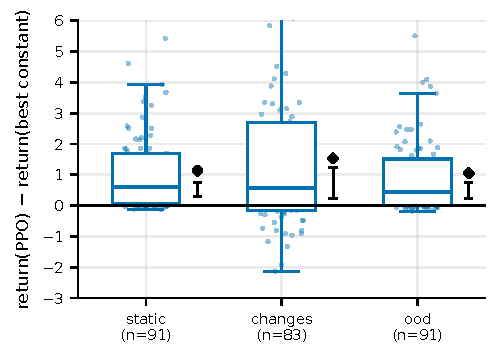
\includegraphics[width=\columnwidth]{fig_paired_conf.pdf}
\caption{Simulation, confirmatory seeds 60000--60099, feasible scenarios: paired return difference of the validation-selected residual PPO (v3) to the best constant, per regime. Box: median and interquartile range; points: every scenario; right of each box: median with $95\,\%$ bootstrap interval (bar) and mean (diamond). Positive is better than the constant.}
\label{fig:paired}\end{figure}

\subsection{How much of the oracle headroom is captured?}\label{sec:headroom}
The hindsight oracle improves on the best constant by $\ConfThreeStaticOrcAbs$, $\ConfThreeChangesOrcAbs$ and $\ConfThreeOodOrcAbs$ mean return in the three regimes ($\ConfThreeStaticOrcPct$, $\ConfThreeChangesOrcPct$ and $\ConfThreeOodOrcPct\,\%$ of $|$return$|$). The selected residual PPO captures $\ConfThreeStaticCap$, $\ConfThreeChangesCap$ and $\ConfThreeOodCap\,\%$ of that headroom; averaged over the three training seeds it captures $\ConfThreeStaticCapMean$, $\ConfThreeChangesCapMean$ and $\ConfThreeOodCapMean\,\%$, and one seed captures less than nothing in the changes regime (Fig.~\ref{fig:headroom}). The learned policy is therefore far from the ceiling for a scenario-aware tuner, most clearly when the payload and target change.

\begin{figure}[t]\centering
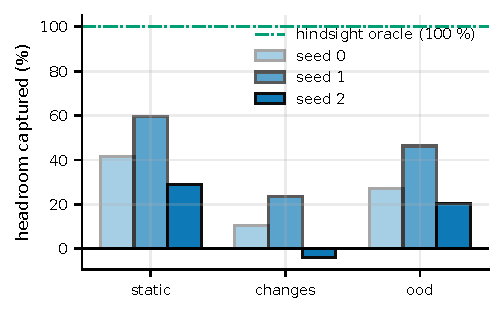
\includegraphics[width=\columnwidth]{fig_headroom.pdf}
\caption{Simulation, confirmatory seeds: headroom captured per training seed, i.e.\ the mean return gain of the policy over the best constant divided by the gain of the hindsight oracle (dashed line: oracle, $100\,\%$), feasible scenarios.}
\label{fig:headroom}\end{figure}

\subsection{Infeasible scenarios}
Infeasible scenarios (margin $<1$ at any point) are $\ConfThreeStaticNInf$, $\ConfThreeChangesNInf$ and $\ConfThreeOodNInf$ of $100$ in the three regimes on the confirmatory seeds. No controller can hold these targets; the policy is not better than the best constant there (changes regime: mean return $\ConfThreeChangesInfPpo$ against $\ConfThreeChangesInfBase$, oracle $\ConfThreeChangesInfOrc$; Table~\ref{tab:infeasible}). They are excluded from the headline tables.

\begin{table}[t]
\centering
\small
\caption{Infeasible scenarios (torque margin $<1$ at any point), confirmatory seeds 60000--60099: mean return. No controller can hold these targets; differences are not evidence of better control.}
\label{tab:infeasible}
\begin{tabular}{lrrrr}
\toprule
Controller & static & changes & ood & \\
\midrule
Tuned preset & $-$40.4 & $-$92.7 & $-$35.8 & \\
Bandit (one-shot) & $-$38.2 & $-$84.2 & $-$34.9 & \\
Best constant & $-$39.5 & $-$85.5 & $-$35.5 & \\
PPO residual (selected) & $-$38.5 & $-$85.2 & $-$35.0 & \\
Hindsight oracle & $-$37.7 & $-$42.6 & $-$34.7 & \\
\midrule
$n$ infeasible & 9 & 17 & 9 & \\
\bottomrule
\end{tabular}
\end{table}


\subsection{v4: a smaller residual range, and SAC and TD3}\label{sec:v4}
On the unseen seeds $70000$--$70099$ PPO with the smaller range gave median differences of $\VFourPpoStaticMed$ (static) and $\VFourPpoOodMed$ (ood), but seed 0 was worse than the constant in both and the changes regime was inconclusive ($\VFourPpoChangesMed$, mean $\VFourPpoChangesMean$, IQR [$\VFourPpoChangesQone$, $\VFourPpoChangesQthree$]); the benefit is smaller than in v3 and the seed sets differ, so we do not conclude that the smaller range is better or worse. \textbf{SAC is mixed:} in the static regime the selected seed's median difference is $\VFourSacStaticMed$ [$\VFourSacStaticLo$, $\VFourSacStaticHi$], an interval that excludes zero, but the paired Wilcoxon test is not significant (Holm-adjusted $p=\VFourSacStaticSeedAHolm$), the mean is $\VFourSacStaticMean$ and the interquartile range [$\VFourSacStaticQone$, $\VFourSacStaticQthree$] straddles zero; the other two seeds are $\VFourSacStaticSeedBMed$ and $\VFourSacStaticSeedCMed$, and all three SAC seeds are worse than the constant when payload and target change. \textbf{TD3 did not beat the constant} (static median $\VFourTdStaticMed$, changes $\VFourTdChangesMed$). SAC and TD3 selected early checkpoints and degraded afterwards (validation degradation up to $\VFourSacValDegA$ and $\VFourTdValDegB$ return units, against at most $\VFourPpoValDegC$ for PPO). No policy helped in the changes regime in v4 (Table~\ref{tab:v4}, Fig.~\ref{fig:algos}).

\begin{table*}[t]
\centering
\small
\caption{Experiment v4 (smaller residual range; PPO, SAC, TD3), unseen seeds 70000--70099, feasible scenarios. Paired return difference to the best constant for the validation-selected seed: median [95\,\% CI] / mean [95\,\% CI] / IQR, and the three per-seed medians. $p_{\mathrm{Holm}}$ over the secondary family of each algorithm.}
\label{tab:v4}
\begin{tabular}{llrrrr}
\toprule
Algorithm & Regime & $\Delta$ median [95\,\% CI] & $\Delta$ mean [95\,\% CI] & IQR & per-seed medians (s0/s1/s2)\\
\midrule
PPO & static & +0.35 [+0.34, +0.36] & +0.38 [+0.36, +0.40] & [+0.33, +0.39] & $-$0.62 / +0.33 / +0.35\\
 & changes & +0.18 [$-$0.08, +0.43] & $-$0.49 [$-$1.28, +0.18] & [$-$0.52, +0.77] & $-$1.20 / +0.13 / +0.18\\
 & ood & +0.34 [+0.29, +0.36] & +0.31 [+0.14, +0.47] & [+0.25, +0.57] & $-$0.56 / +0.30 / +0.34\\
\midrule
SAC & static & +0.25 [+0.12, +0.32] & +0.05 [$-$0.18, +0.28] & [$-$0.29, +0.41] & +0.25 / +0.08 / $-$0.24\\
 & changes & $-$0.26 [$-$1.14, $-$0.06] & $-$1.57 [$-$2.39, $-$0.86] & [$-$2.37, +0.12] & $-$0.26 / $-$0.97 / $-$1.40\\
 & ood & +0.24 [+0.19, +0.29] & $-$0.03 [$-$0.28, +0.18] & [$-$0.02, +0.37] & +0.24 / +0.07 / $-$0.21\\
\midrule
TD3 & static & $-$0.17 [$-$0.29, +0.09] & +0.17 [$-$0.09, +0.45] & [$-$0.64, +0.54] & $-$1.02 / $-$0.70 / $-$0.17\\
 & changes & $-$2.13 [$-$2.50, $-$1.82] & $-$2.06 [$-$2.91, $-$0.72] & [$-$3.70, $-$1.17] & $-$2.13 / $-$2.38 / $-$1.49\\
 & ood & $-$0.10 [$-$0.26, +0.04] & +0.19 [$-$0.13, +0.54] & [$-$0.66, +0.47] & $-$0.89 / $-$0.70 / $-$0.10\\
\bottomrule
\end{tabular}
\end{table*}


\begin{figure*}[t]\centering
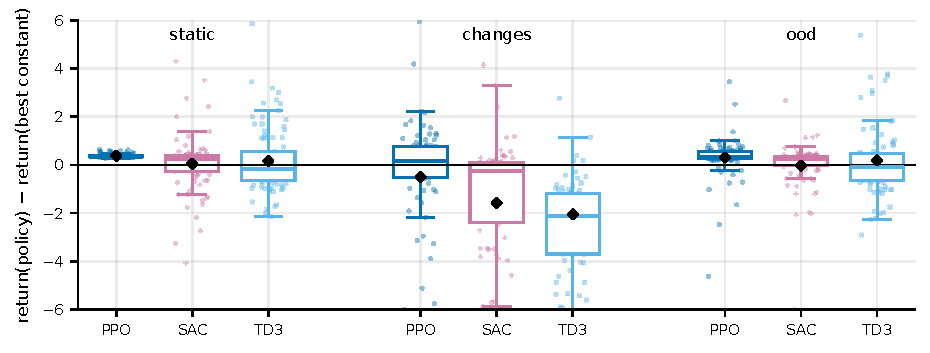
\includegraphics[width=\textwidth]{fig_algos.pdf}
\caption{Simulation, unseen seeds 70000--70099 (v4), feasible scenarios: paired return difference of the validation-selected policy of each algorithm to the best constant, per regime. Box: median and interquartile range, points: scenarios, diamond: mean.}
\label{fig:algos}\end{figure*}

\begin{figure*}[t]\centering
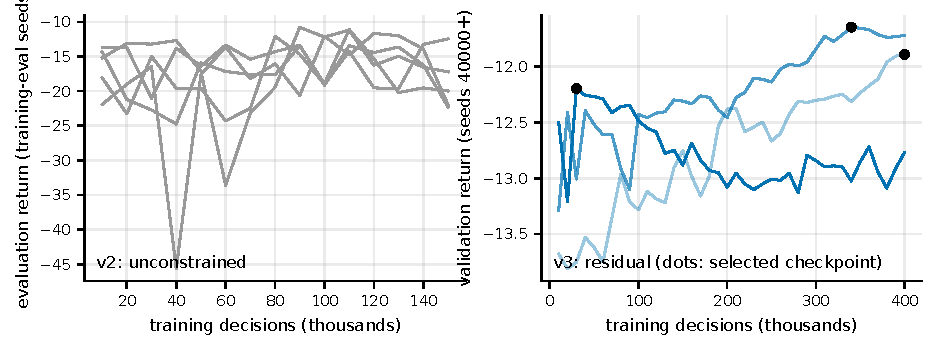
\includegraphics[width=\textwidth]{fig_curves.pdf}
\caption{Simulation. Left: v2 evaluation return on the training-evaluation seeds (five seeds): peak at $60$k--$120$k decisions, then degradation. Right: v3 validation return on seeds 40000+ (three seeds); dots mark the checkpoint selected on validation. The two panels use different evaluation streams and are not the same measurement.}
\label{fig:curves}\end{figure*}

\subsection{Post-hoc check: is the benefit just a better constant?}\label{sec:posthoc}
The learned policies end at gains that vary little across scenarios: in v3 the median final gains are $K_p=\ConfThreeStaticGainKpMed$ ($10$--$90\,\%$ range $\ConfThreeStaticGainKpPlo$--$\ConfThreeStaticGainKpPhi$) and $K_d=\ConfThreeStaticGainKdMed$ in the static regime, against $\ConfThreeStaticGainKpBase$ and $\ConfThreeStaticGainKdBase$ for the best constant; in v4 the PPO gains are almost constant ($K_p=\VFourPpoStaticGainKpMed$, $10$--$90\,\%$ range $\VFourPpoStaticGainKpPlo$--$\VFourPpoStaticGainKpPhi$). This raises the possibility that part or all of the benefit comes from a better constant than the modest search found, not from adaptation. We therefore added, \emph{after} the confirmatory runs and labelled post hoc, two constants derived on validation seeds only: a much larger validation search and the policy's own median gains.
\textbf{[PENDING: results of \texttt{simulation/constant\_sensitivity.py} (\texttt{results/constant\_sensitivity\_v3}); this paragraph and the claim in the abstract must be revised according to them before the draft is polished.]}

\section{Discussion}
\paragraph*{What the evidence supports.} In simulation on the unvalidated twin, a residual PPO around a validation-tuned constant beat that constant by about $0.5$--$0.6$ median return, consistently across three training seeds and on fresh scenarios. But the same data show that most of this gain is available without learning. A larger validation search for the constant recovers $\SensVThreeStaticBestConstantExtBestConstantMed$, $\SensVThreeChangesBestConstantExtBestConstantMed$ and $\SensVThreeOodBestConstantExtBestConstantMed$ of it in the three regimes, and a non-learned rule with three load features matches the policy within noise. The policy's gain over the stronger constant is small ($\SensVThreeStaticPpoBestConstantExtMed$ static, $\SensVThreeChangesPpoBestConstantExtMed$ with changes, $\SensVThreeOodPpoBestConstantExtMed$ out of distribution) and in the payload-change regime not distinguishable from zero. The supported conclusion is therefore protocol-level: \emph{an apparent RL gain over a modestly tuned constant can mostly be a better-tuned constant}, and papers should report a validation-tuned constant with a generous search and a non-learned scenario-conditioned baseline next to any learned tuner.

\paragraph*{Does the policy adapt at all?} Its gains are not constant: the scatter of final gains against scenario parameters (Fig.~\ref{fig:scatter}) shows that $K_p$ is markedly higher when gravity acts (about $27$--$37$ against $22$--$27$), i.e.\ the policy tracks the gravity load, in the way the non-learned rule does. It learned a plausible, simple dependence on the load; it did not learn more than the simple rule captures.

\paragraph*{Why the unconstrained setup failed (hypotheses, not shown).} v2 differed from v3 in four ways at once (unconstrained actions, an under-shaped reward, a checkpoint chosen on the training-evaluation stream, early-peaking training), and the experiments do not isolate which mattered. The gains piled up at the bounds, suggesting that without a reference the policy exploits the cost structure at the edges of the action range.

\paragraph*{Mean versus median.} Medians and means of the paired differences can disagree: on the confirmatory seeds the one-shot bandit is slightly below the best constant in the median in the static regime ($\ConfThreeStaticBanditMed$) but above it in the mean ($\ConfThreeStaticBanditMean$), because a minority of scenarios with large gains dominate the mean. This is why median, mean and interquartile range are reported side by side and why a median interval alone should not be read as an effect size for the mean.

\paragraph*{Headroom.} The hindsight oracle is far ahead of every deployable method (the policy captured $\ConfThreeStaticCapMean$, $\ConfThreeChangesCapMean$ and $\ConfThreeOodCapMean\,\%$ of its headroom on average over seeds), so there is room for scenario-aware tuning; the evidence here is that neither this PPO configuration nor a simple load-conditioned rule reaches it.

\paragraph*{Practical guidance.} Report (i) a validation-tuned constant with a search budget at least as large as the learner's, (ii) a non-learned scenario-conditioned baseline, (iii) a hindsight oracle, (iv) infeasible scenarios separately, and (v) paired differences with median, mean and spread. Treat success-rate gains with suspicion unless they replicate across seed sets.

\section{Limitations and Threats to Validity}
\begin{itemize}
\item \textbf{Unvalidated twin; no hardware.} Parameters come from a datasheet with a documented inconsistency; nothing has been compared with a measured response. Every statement is conditional on the twin.
\item \textbf{One motor model, one payload family, one reward design, three seeds per algorithm} (five for v2). Between-seed spread is reported, but three seeds give little power for seed-level claims; the changes regime in particular rests on two of three seeds after Holm correction.
\item \textbf{Baseline strength.} The best constant is found with a modest validation search (about $50$ candidates); a stronger search might close part of the gap (Section~\ref{sec:posthoc}). The oracle is an upper bound chosen with hindsight and is not a deployable method.
\item \textbf{Design chosen after seeing results.} The v3 design followed the v2 test results on seeds 50000+; only seeds 60000+ are confirmatory for v3, and v4 (seeds 70000+) is a separate experiment. There is no formal pre-registration file for the RL runs.
\item \textbf{Metrics and success definition.} Return is a composite with hand-set weights; the ranking could change with the weights (not studied). The success rate is descriptive and was not stable across seed sets.
\item \textbf{Modelling.} Inductance is zero in the base twin, the gearbox is ideal, friction is small, and there is no thermal model; the feasibility margin is an upper bound that ignores back-EMF.
\item \textbf{Reproducibility scope.} The PPO, SAC and TD3 policies are provided as committed weight files and are not retrained by the comparison scripts. The numpy bandit policy retrains byte-identically only on the same NumPy and Python build (an independent check across two platforms found a largest weight difference of $7.3\times10^{-4}$ with the same metrics).
\item \textbf{Extension.} Nothing here supports statements about industrial robot joints; extending the claims would need hardware data on the intended joint class.
\end{itemize}

\section{Conclusion and Future Work}
In simulation on an unvalidated digital twin, a PPO policy acting as a residual on a validation-tuned constant beat that constant by about $0.5$--$0.6$ median return across training seeds and on fresh scenarios, while capturing a minority of the hindsight-oracle headroom; an unconstrained setup, TD3 and (mostly) SAC did not reproduce the benefit. [Revise after the post-hoc constant-sensitivity result.] Next steps, in order: finish the post-hoc check and a stronger constant baseline; more seeds and a second motor model; reward-weight sensitivity; and the hardware replication protocol of Appendix~\ref{app:hardware}, which would be the first test of any of these claims against measurements.

\section*{Availability}
Code, committed policy weights with SHA-256 hashes (\texttt{rl/policies/}), per-episode results (\texttt{results/*/per\_episode.csv}) and the scripts that regenerate every number, table and figure of this draft (\texttt{paper/make\_numbers.py}, \texttt{tables.py}, \texttt{figures.py}; \texttt{make -C paper all}) are in the project repository; the repository URL, the archived release and any DOI will be added by the authors at submission. Reproduction needs the pinned requirements and the RL extras (\texttt{requirements-rl.txt}). A venue-specific statement on the use of AI assistance in writing and coding must be added following the target venue's policy.


\bibliographystyle{IEEEtran}
\bibliography{../refs}

\appendices
\section{Hardware Replication Protocol and Plan (no results)}\label{app:hardware}
\textbf{This appendix is a plan. No hardware experiment has been run and no measured value appears anywhere in this paper.} The motor, bench and measurement choices are still open; the protocol below is written so that another laboratory can run it and so that the claims of the main text can be tested.

\paragraph*{Purpose.} (i) Measure the quantities the twin takes from a datasheet (armature resistance, back-EMF constant, no-load speed and current, viscous and Coulomb friction, reflected inertia, gearbox efficiency); (ii) compare measured and simulated closed-loop step responses for the gain sets used here; (iii) test whether a policy trained on the twin transfers without retraining and whether the residual benefit over a tuned constant, if any, survives.

\paragraph*{Planned protocol outline (to be detailed in a replication kit).}
\begin{enumerate}
\item \emph{Rig characterisation:} sampling-time jitter, encoder resolution and repeatability, supply sag under load, current-sense accuracy.
\item \emph{Static identification:} steady speed and current versus voltage (several voltages, both directions, repeated), locked-rotor current with a duty-limited protocol.
\item \emph{Dynamic identification:} voltage steps, pseudo-random binary excitation, coast-down; fit with a parameter-identifiability analysis (parameters flagged as not identifiable are reported, not forced).
\item \emph{Closed-loop validation:} step responses for the fixed gain sets and targets used in the simulation study; compare with the twin using pre-set pass thresholds on normalised error, overshoot and settling.
\item \emph{Payload and gravity:} measure with and without a payload arm, including a condition near the torque-feasibility boundary.
\item \emph{Tuner comparison on hardware:} best constant versus the learned residual policy and the baselines on the same trials, paired, with randomised order.
\item \emph{Repeatability:} several sessions, and at least one independent unit or laboratory.
\end{enumerate}

\paragraph*{What must be fixed before any data are taken.} The hypotheses, the numerical thresholds (equivalence margins, validation thresholds, the number of trials) and the exclusion rules go into a pre-registration file committed before the first confirmatory run, with the reasons for each threshold (engineering relevance, measurement resolution or pilot data). The safety checklist (current limit, guarded shaft, no locked rotor at full voltage, emergency stop) must be signed by the person running the rig; this paper does not provide instructions for unsafe operation.

\paragraph*{Claims ladder.} Until measured data exist, results are worded ``in simulation''; ``validated'' is used only for quantities that passed stated thresholds on measured data; multi-unit or multi-laboratory statements require replication data; and nothing is said about industrial joints from a small hobby-class motor.

\section{Supplement: seed sets, baselines and settings}\label{app:supplement}
\begin{table}[t]\centering\small
\caption{Seed sets. Every comparison folder under \texttt{results/} states its set in its manifest.}\label{tab:seedsets}
\begin{tabular}{lll}\toprule
Seeds & Used for & Status\\\midrule
$<20000$ & training, training-evaluation stream $10000+s$ & --\\
$40000$--$40039$ & best constant, checkpoint (first $30$), policy-seed selection & validation\\
$50000$--$50099$ & v2 comparison; v3 comparison & exploratory for v3\\
$60000$--$60099$ & v3 comparison (run once) & confirmatory (v3)\\
$70000$--$70099$ & v4 comparisons (run once) & confirmatory (v4)\\
$80000$--$80099$ & post-hoc sensitivity analysis (stronger baselines derived on validation seeds; run once) & fresh, post hoc\\\bottomrule
\end{tabular}\end{table}

\begin{table}[t]\centering\small
\caption{Tuning methods: information used and tuning budget.}\label{tab:baselines}
\begin{tabular}{p{2.3cm}p{2.7cm}p{2.7cm}}\toprule
Method & Information & Budget\\\midrule
Tuned preset, legacy & none (fixed) & hand-found, once\\
Ziegler--Nichols & linearised nominal plant for the load & closed-form\\
Bandit (one-shot, re-queried) & scenario context & REINFORCE training on the twin\\
Best constant & none at run time & about $50$ candidates $\times$ $40$ validation scenarios per regime\\
Residual PPO/SAC/TD3 & 16-dim.\ observation every $20$\,ms & $150$k--$400$k decisions $\times$ seeds; checkpoint on validation\\
Hindsight oracle & the outcome (not deployable) & $48$ random + $20$ grid + $3$ per scenario\\\bottomrule
\end{tabular}\end{table}

\begin{table}[t]
\centering
\small
\caption{RL experiments: settings that differ between versions. Common: Stable-Baselines3 PPO, decision every 20\,ms over a 2\,s episode, 16-dimensional observation, reward weights from the YAML (error 1.0, effort 0.02, chatter 0.5, gain change 0.02, overshoot 2.0).}
\label{tab:hparams}
\begin{tabular}{llll}
\toprule
 & v2 & v3 & v4\\
\midrule
Action space & multiplicative, $\pm10\,\%$ / decision & residual, $\times2^{a}$ (Ki: $+20a$) & residual, $\times1.5^{a}$ (Ki: $+10a$)\\
Decisions per seed & 150000 & 400000 & 200000\\
Seeds & 5 & 3 & 3\\
Learning rate (PPO) & 0.0003 & 0.0001 & 0.0001\\
PPO log-std init & default (0) & -1.0 & -1.0\\
Training reward extra term & none & time outside 2\,\% band ($w=1$) & same as v3\\
Checkpoint used & best on training-eval seeds & best on validation seeds 40000+ & best on validation seeds 40000+\\
Net architecture & 64--64 & 64--64 & 64--64\\
\bottomrule
\end{tabular}
\end{table}

\begin{table*}[t]
\centering
\small
\caption{Exploratory result (v3, seeds 50000--50099; the design was chosen after seeing v2 results on these seeds). Same layout as Table~\ref{tab:main_conf}.}
\label{tab:main_expl}
\begin{tabular}{llrrrrrr}
\toprule
Regime & Controller & Return, mean $\pm$ SD & $\Delta$ median [95\,\% CI] & $\Delta$ mean [95\,\% CI] & IQR of $\Delta$ & $p_{\mathrm{Holm}}$ & Success (desc.)\\
\midrule
static (n=94) & Tuned preset & $-$11.60 $\pm$ 9.10 & $-$2.61 [$-$3.88, $-$1.69] & $-$3.66 [$-$4.41, $-$2.95] & [$-$5.74, $-$1.00] & $1.7{\times}10^{-13}$ & 13\,\%\\
 & Bandit (one-shot) & $-$7.95 $\pm$ 8.14 & $-$0.16 [$-$0.24, $-$0.05] & $-$0.02 [$-$0.27, +0.26] & [$-$0.39, +0.16] & 0.148 & 63\,\%\\
 & Bandit (re-tuned) & $-$7.95 $\pm$ 8.14 & $-$0.16 [$-$0.24, $-$0.05] & $-$0.02 [$-$0.27, +0.26] & [$-$0.39, +0.16] & 0.148 & 63\,\%\\
 & Best constant & $-$7.93 $\pm$ 8.11 & -- & -- & -- & ref. & 54\,\%\\
 & PPO residual (selected) & $-$7.10 $\pm$ 7.97 & +0.50 [+0.30, +0.83] & +0.83 [+0.66, +1.02] & [+0.10, +1.48] & primary: $1.3{\times}10^{-14}$ & 74\,\%\\
 & Hindsight oracle & $-$6.53 $\pm$ 7.99 & +0.81 [+0.68, +1.11] & +1.40 [+1.16, +1.67] & [+0.48, +1.94] & $1.1{\times}10^{-15}$ & 85\,\%\\
\midrule
changes (n=89) & Tuned preset & $-$28.79 $\pm$ 27.31 & $-$5.71 [$-$7.29, $-$3.64] & $-$7.48 [$-$9.45, $-$5.77] & [$-$10.46, $-$1.75] & $1.9{\times}10^{-12}$ & 16\,\%\\
 & Bandit (one-shot) & $-$20.19 $\pm$ 23.63 & +0.32 [+0.11, +0.89] & +1.13 [+0.54, +1.74] & [$-$0.07, +1.53] & $6.3{\times}10^{-5}$ & 45\,\%\\
 & Bandit (re-tuned) & $-$20.49 $\pm$ 23.42 & +0.04 [$-$0.36, +0.33] & +0.82 [+0.20, +1.50] & [$-$0.78, +1.11] & 1.000 & 49\,\%\\
 & Best constant & $-$21.32 $\pm$ 23.93 & -- & -- & -- & ref. & 34\,\%\\
 & PPO residual (selected) & $-$19.84 $\pm$ 24.57 & +0.55 [+0.25, +1.49] & +1.47 [+0.56, +2.55] & [$-$0.15, +2.66] & $9.0{\times}10^{-5}$ & 44\,\%\\
 & Hindsight oracle & $-$13.94 $\pm$ 13.14 & +2.22 [+1.38, +3.74] & +7.37 [+4.74, +10.59] & [+0.69, +6.55] & $6.1{\times}10^{-15}$ & 58\,\%\\
\midrule
ood (n=94) & Tuned preset & $-$14.03 $\pm$ 14.51 & $-$2.07 [$-$3.47, $-$1.02] & $-$3.61 [$-$4.59, $-$2.65] & [$-$5.06, $-$0.14] & $1.0{\times}10^{-10}$ & 23\,\%\\
 & Bandit (one-shot) & $-$10.34 $\pm$ 13.11 & $-$0.09 [$-$0.15, $-$0.05] & +0.08 [$-$0.13, +0.30] & [$-$0.25, +0.29] & 1.000 & 63\,\%\\
 & Bandit (re-tuned) & $-$10.34 $\pm$ 13.11 & $-$0.09 [$-$0.15, $-$0.05] & +0.08 [$-$0.13, +0.30] & [$-$0.25, +0.29] & 1.000 & 63\,\%\\
 & Best constant & $-$10.42 $\pm$ 13.07 & -- & -- & -- & ref. & 49\,\%\\
 & PPO residual (selected) & $-$9.36 $\pm$ 12.83 & +0.57 [+0.26, +0.96] & +1.06 [+0.81, +1.34] & [+0.07, +1.84] & $1.2{\times}10^{-11}$ & 69\,\%\\
 & Hindsight oracle & $-$8.39 $\pm$ 12.74 & +0.94 [+0.82, +1.29] & +2.03 [+1.54, +2.61] & [+0.60, +2.30] & $1.1{\times}10^{-15}$ & 85\,\%\\
\bottomrule
\end{tabular}
\end{table*}


\end{document}
